\documentclass[t]{beamer}
\usepackage[portuguese]{babel}
\usepackage[utf8]{inputenc}
\usetheme{Berkeley}
\usecolortheme{seahorse}

\addto\captionsportuguese{
	\renewcommand{\figurename}{Fig.}
	\renewcommand{\tablename}{Tab.}
}

\title{Introdução à Internet das Coisas}
\subtitle{Seu panorama atual: Uma visão da área do ponto de vista acadêmico e empresarial}

\AtBeginSection[]
{
	\begin{frame}
	\frametitle{Sumário}
	\tableofcontents[currentsection]
\end{frame}
}

\begin{document}

\frame{\titlepage}

\begin{frame}
\frametitle{Sumário}
\tableofcontents
\end{frame}

\section{O que é IoT?}

\begin{frame}
\frametitle{O que é Internet das Coisas}

\begin{itemize}
	\item Mais uma \textit{buzzword}?!
	\item Coisas conectadas à Internet?!
	\item Dados de coisas pela Internet?!
	\item Análise de dados de coisas conectadas?!
	\item Processamento de dados de coisas conectadas?!
	\item \textbf{Informações e ações inteligentes tomadas a partir da análise e processamento de dados de coisas conectadas à Internet!!}
\end{itemize}
\end{frame}

\begin{frame}
	\frametitle{O que é Internet das Coisas}
	\begin{figure}
		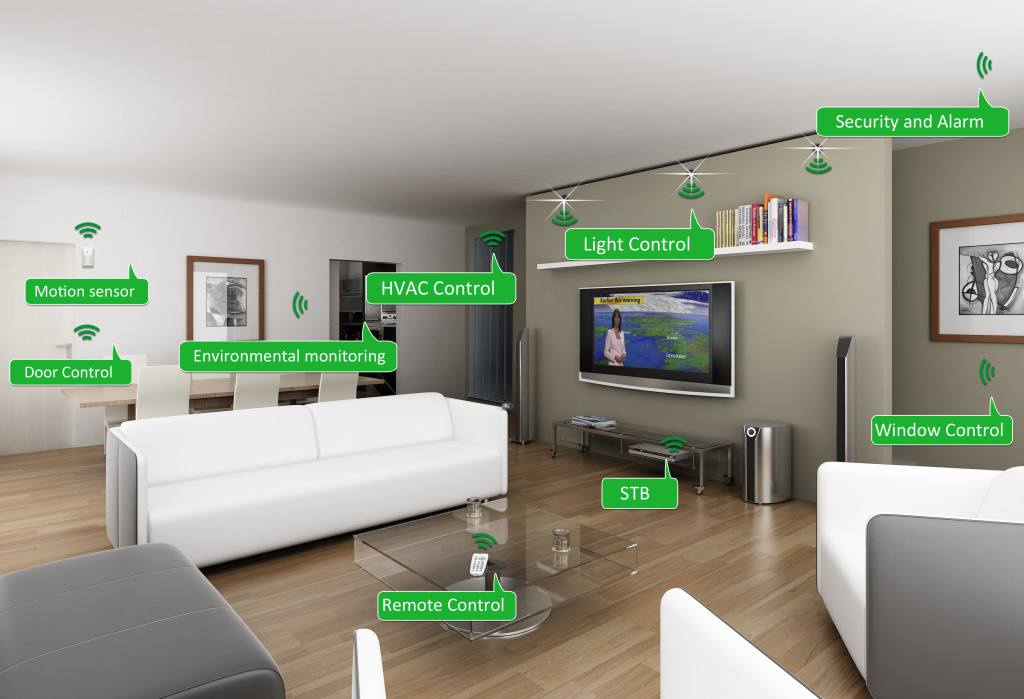
\includegraphics[width=0.9\textwidth]{home-automation-google-brillo-os-1-1024x699}
	\end{figure}
	\scriptsize Fonte: Google Brillo OS para IoT - Toobler.com\\
	\tiny \url{www.toobler.com/blog/google-provides-a-customized-os-for-internet-of-things-iot-brillo}
\end{frame}

\begin{frame}
	\frametitle{O que é Internet das Coisas}
	\begin{figure}
		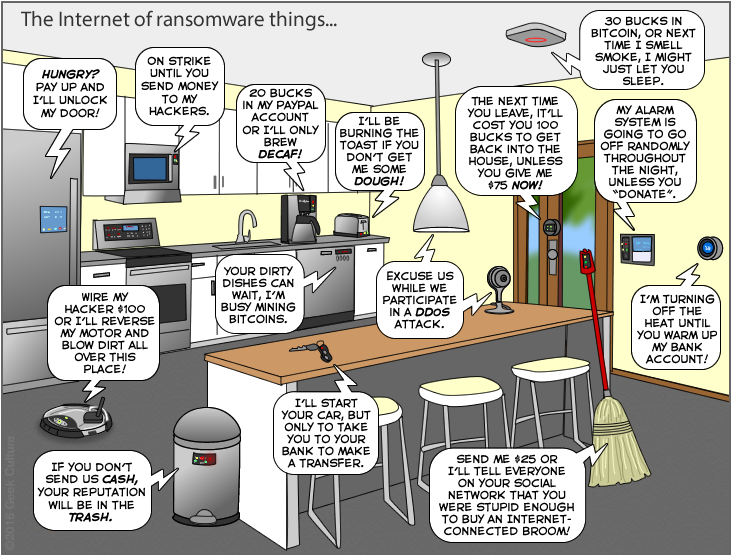
\includegraphics[width=0.85\textwidth]{thejoyoftech-geekculture}
	\end{figure}
	\scriptsize Fonte: The Internet of ransomeware things... - Nitrozac \& Snaggy\\
	\tiny \url{www.geekculture.com/joyoftech/joyarchives/2340.html}
\end{frame}

\section{Histórico}

\begin{frame}
\frametitle{Fatos Históricos}

Adoção da telemetria pelo exército
\begin{itemize}
	\item 1967 - REMBASS Remotely Monitored Battlefield Sensor System
	\item 1978 - Lincoln Labs Distributed Sensor Networks for Aircraft Detection
\end{itemize}

Conceitos fundamentais de pesquisa

\begin{itemize}
	\item 1992 - RAND Workshop  - Future Tech, including Smart Dust
	\item 1994 - UCLA Low Power Wireless Integrated Microsensors
	\item 1997 - Smart Dust proposal put forward by Kris Pister, Berkeley
	\item 1998 - RFC 2460 define IPv6 with 128 bits
	\item 1999 - PicoRadioProject started by Jan Rabaey(Berkeley)
\end{itemize}

\end{frame}

\begin{frame}
\frametitle{Fatos Históricos}
Visão comercial emergente

\begin{itemize}
	\item 1999 - Kevin Ashton coins “Internet of Things” whilst working on RFID
	\item 2000 - Crossbow starts selling proprietary Berkeley motes
	\item 2002 - Dust, Ember, Sensicast, etc founded
\end{itemize}

\end{frame}

\begin{frame}
\frametitle{Fatos Históricos}

Onda de padrões de conectividade

\begin{itemize}
	\item 2003 - IEEE 802.15.4 standard founded (foundation of Zigbee)
	\item 2006 - Zigbee ratified, and chips being sold
	\item 2007 - WirelessHARTratified, IETF 6LoWPAN published
	\item 2008 - IETF ROLL RPL \& ETSI M2M started, among many others
\end{itemize}

Segunda onda de tecnologias de conectividade

\begin{itemize}
	\item 2010 - LPWANs start to emerge such as Sigfox (later Lora)
	\item 2011 - IPv6 is public
	\item 2016 - 3GPP R13 NB-IoT is standardised
\end{itemize}

\end{frame}

\begin{frame}
	\frametitle{Referências}
	Parte desses fatos históricos foram retirados da apresentação do Mischa Dohler sobre Smart Cities na \textit{São Paulo School of Advanced Science on Smart Cities}\\
	\bigskip
	\scriptsize Fonte: São Paulo School of Advanced Science on Smart Cities\\
	\tiny \url{interscity.org/advanced-school}
\end{frame}

\section{Arquiteturas}

\begin{frame}
	\frametitle{Arquitetura proposta pela Intel para Internet das Coisas}
	\begin{figure}
		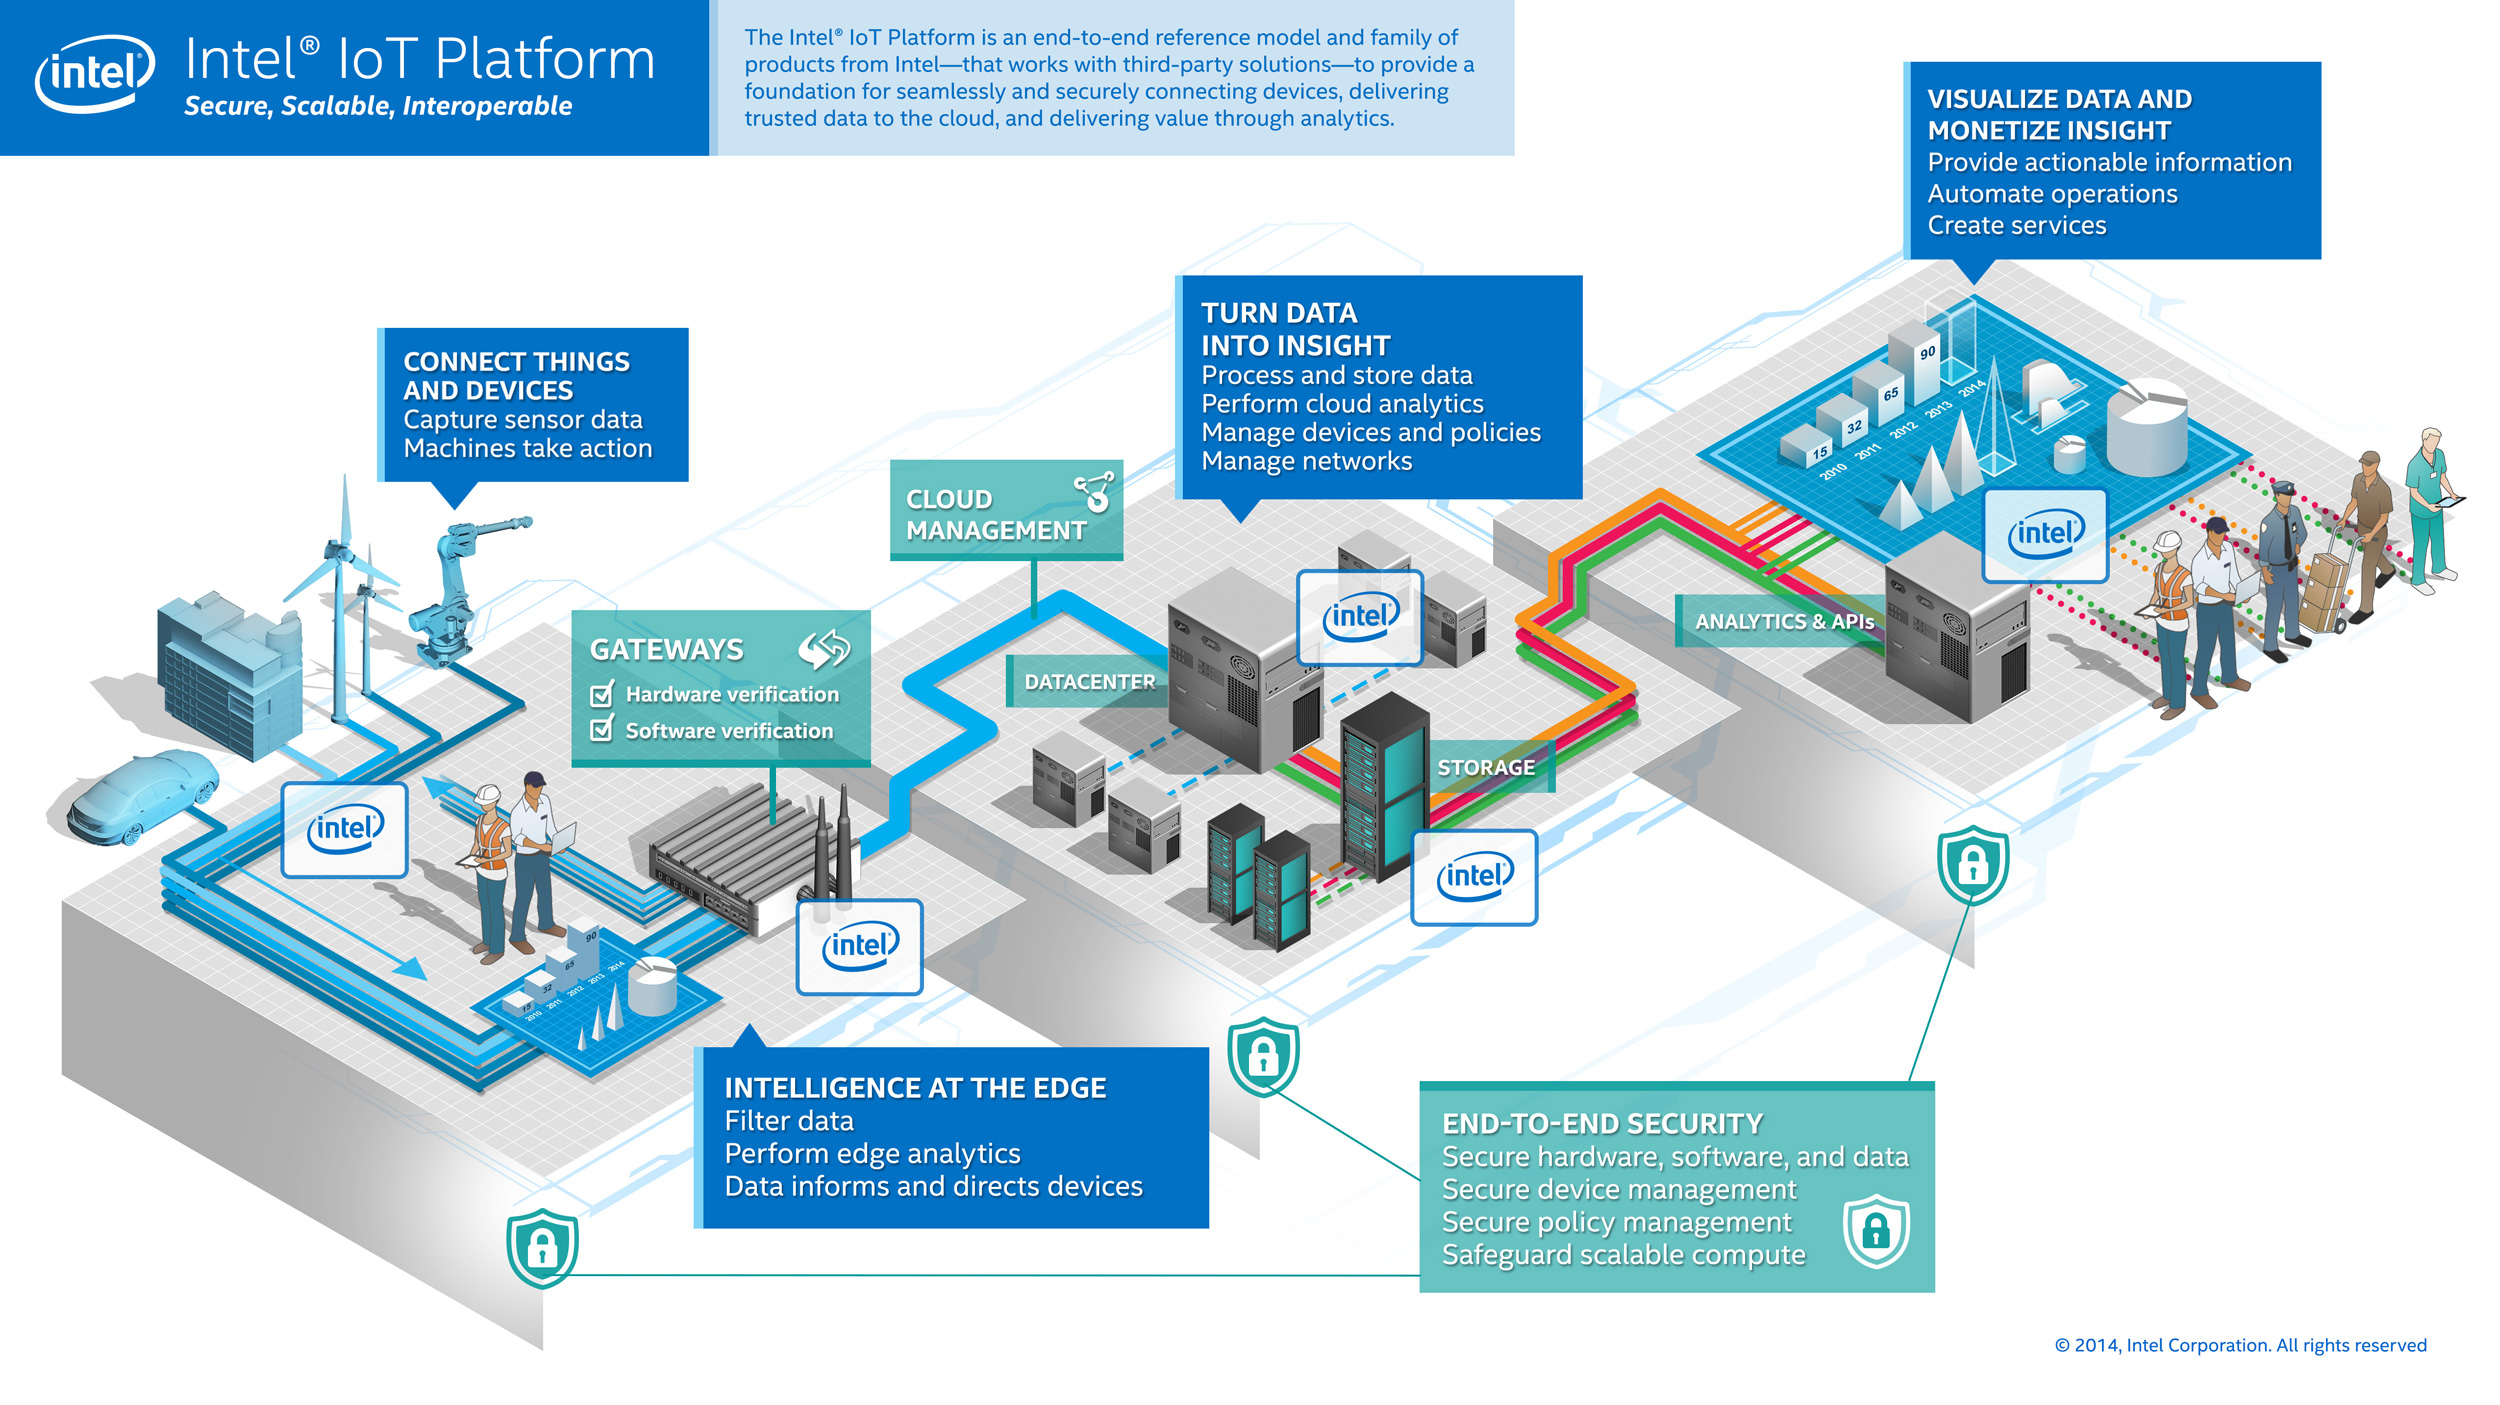
\includegraphics[width=0.9\textwidth]{inteliotplatform}
	\end{figure}
	\scriptsize Fonte: Intel Corp.\\
	\tiny \url{software.intel.com/en-us/iot/}
\end{frame}

\begin{frame}
\frametitle{Arquitetura proposta pela IBM para Internet das Coisas}
\begin{figure}
	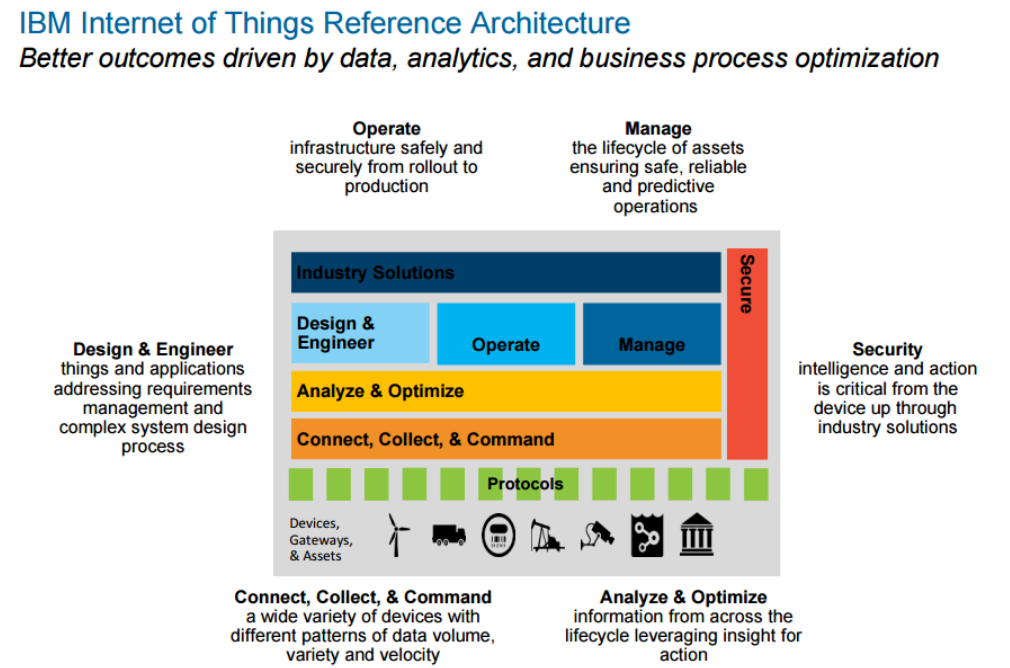
\includegraphics[width=0.9\textwidth]{arquiteturaiotibm}
\end{figure}
\scriptsize Fonte: IBM
\end{frame}

\section{Contextos}

\begin{frame}
	\frametitle{Ciência de contexto para Internet das Coisas}
	\begin{figure}
		\centering
		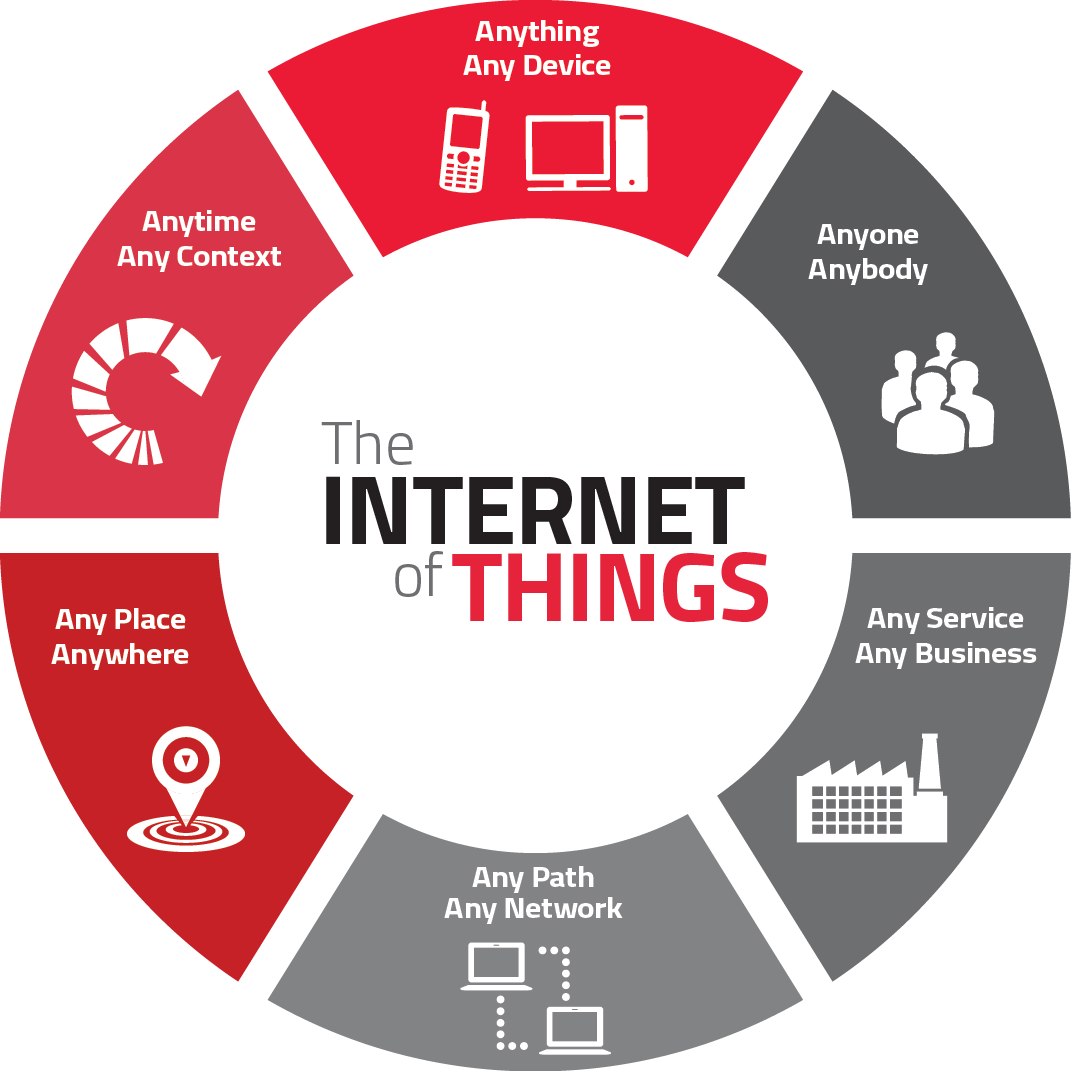
\includegraphics[width=0.7\linewidth]{contextosdeiot}
	\end{figure}	
\end{frame}

\begin{frame}
	\frametitle{Ciência de contexto para Internet das Coisas}
	O que é preciso levar em consideração em uma solução básica?!
	\begin{itemize}
		\item Consumo
		\item Conectividade
		\item Comunicação
		\item Custo
		\item Conscientização
	\end{itemize}
\end{frame}

\frame{\titlepage}

\end{document}
